\documentclass[runningheads]{llncs}

\usepackage[T1]{fontenc}

\usepackage{graphicx}

\usepackage{hyperref}[colorlinks,linkcolor=blue]

\begin{document}
	\title{Seminar- scientific methods in information systems}
	\subtitle{Predictive Process Monitoring Methods:\\ Which One Suits Me Best?}
	\author{Shuaiwei YU \inst{1} }
	\institute{Technical University of Munich\\
	\email{shuaiwei.yu@tum.de}}
	\maketitle
	
	%here begins the abstract
	\begin{abstract}
		The abstract should briefly summarize the contents of the paper in
		150--250 words.

		\keywords{predictive process monitoring  \and literature review \and algorithm.}
	\end{abstract}
	
	%the first part: Introduction into the topic
	\section{Introduction}
	Predictive Process Monitoring (PPM) or Predictive Business Process Monitoring (PBPM) is known as a specific brach of process mining. Unlike process mining XXXXX\cite{}, the predictive monitoring makes prediction about the development of uncompleted business instances at runtime with given input data. 
	
	%TODO: PPM的好处
	%TODO: PPM好处举例子
	
	%TODO: PPM需要的数据 event log 等等
	
	%TODO: 写这篇文章的动机
	
	
	The remainder of this article is developed as follows. Section 2 recorded the systematic literature review protocol, section 3 reveals the results of systematic literature review, section 4 searches on the trend of predictive process monitoring, and section 5 makes a conclusion about the article. 
	
	%the second part: Systematic Literature Review Protocol
	\section{Systematic Literature Review Protocol}
		%overview of the literature review.
		The research questions are formulated in the systematic literature review protocol, the search protocol is defined, and the selection criteria are developed. The selection criteria are based on the selection criterion of \cite{original} and are modified following the guideline provided in Kitchenham's article \cite{guidline}. The work consisted of several stages. In the first stage, The review protocol was designed. Specifically, the research questions to be investigated were formulated, and I chose the electronic database that will be used to run the search. The selection criteria, as well as inclusion criteria, were also defined. In the next stage, the horizontal search was run. The documents acquired were then filtered according to selection criteria; in the end, the final list of documents will be generated.
		
		%research questions development.
		The main research question (\textbf{RQ}):"\textit{What is the development and trend of the predictive process monitoring techniques over the research period?}" can be decomposed in four sub-question as follows. The first two sub-questions are so developed in order to research the current trends and algorithmic distribution of the predictive process monitoring. \textbf{RQ1}: "\textit{What is the distribution of the literature about predictive process monitoring over the search period?}" and \textbf{RQ2}: "\textit{What aspects can be predicted by the predictive process monitoring?}". The next sub-question focuses on the aspects of outcome that can be predicted, \textbf{RQ3}:"\textit{What is the distribution of the algorithms used in predictive process monitoring over the search period?}". In the last question, I want to research the reason that leads to the current trend of predictive process monitoring, i.e., \textbf{RQ4}: "What leads to the trend of predictive process monitoring?"
		
		%motivations of the research questions.
		In the first research question, I want to visualize the distribution of the article published in order to analyze the current trend of predictive process monitoring. With this visualization, people are able to take a deeper look into the development of interest in the industry of predictive process monitoring. The second research question examines the distribution of algorithms used for predictive process monitoring. The motivation for this is that I want to reveal which algorithms are more popular and widely used. With the first two research questions, current research trend of predictive process monitoring can be derived. I can also analyze the possible research gaps where further academic contributions could be made. In \cite{original}, several aspects were already listed. However, the third research questions want to research whether there are new predictive aspects developed or how the new predictive process monitoring model predicts these aspects differently. The last research question tries to look into the reason that led to the current development of predictive process monitoring so that I might predict what the research direction of this field might be.
		
		%development of search string
		To develop the search string, I followed the guidelines and suggestions given by \cite{guidline} and based on the work of \cite{original}, The first search string I use is: ("predictive" OR "prediction") + ("business process" OR "process mining"). Furthermore, in order to explore as many results as possible, I also decided another search string: ("predictive" OR "prediction") + "process monitoring". 
		
		%electronic database
		After defining the search string, I could choose electronic databases for searching. I decided to use Google Scholar as electronic databases to be used, for its completeness and simple operability. The search period was between year 2018 and 2022.
		
		%steps of filtering below
		The first step of the filtering is about identifying the duplicates. Since several Databases are used, and the keywords can potentially overlap, our goal is to identify the literature that appeared more than once and whose name and author are identical. Only one of the papers will be preserved for future processes. In the next step, I look into the title of the papers gathered. In this step, (i) the studies that are related to a different field will be removed (e.g., "A Chemical Monitoring and Prediction System in Semiconductor Manufacturing Process Using Bigdata and AI Techniques", or "Condition monitoring and prediction of solution quality during a copper electroplating process"); (ii) the documents which are not proper research papers should also be removed (e.g., "Integration of an Explainable Predictive Process Monitoring System into IBM Process Mining Suite (Extended Abstract)").
				
		%The last steps of filtering
		Moreover, I only consider the papers published in conferences, journals, and workshops, because, in comparison to degree thesis, published articles are more professional and have a higher academic contribution. In the next step of filtering, I looked into the abstract of each paper in order to evaluate its relevance. I also leave out the position paper at this stage since I only intended to look into the algorithms being used. In the last stage, I use the inclusion criterion \textit{"the study should propose a novel algorithm or technique for predictive process monitoring"} to further select the papers used for our study.
		
		%clarification of the table
		The following table summarizes a specific list of my literature search. Out of 263 hits, I performed the filtering as listed above-mentioned, and according to selection criteria, I selected 28 papers. 4 more articles were added via vertical search. \footnote{The queries were run on 18th May 2022}

		\begin{figure}
		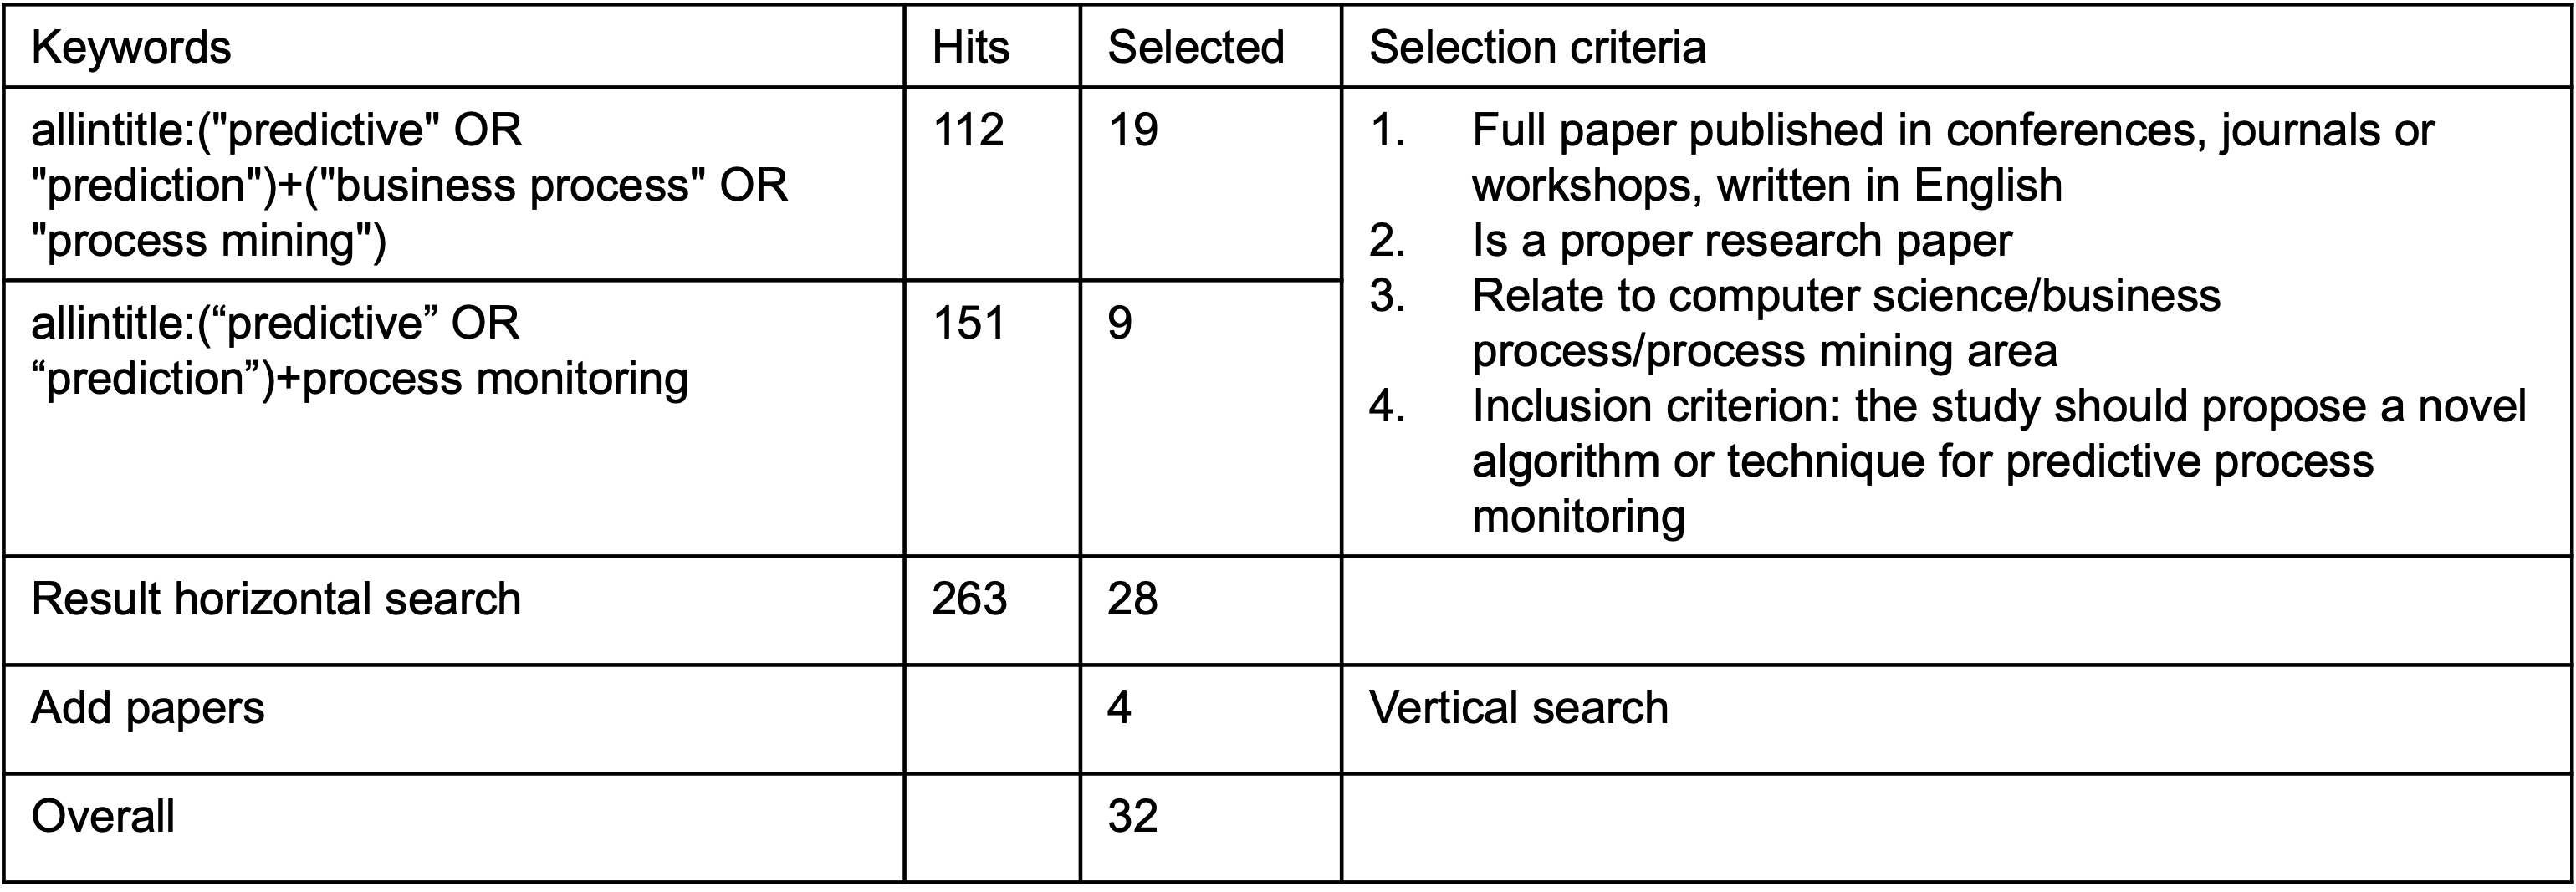
\includegraphics[width=\textwidth]{Filtering.png}
		\caption{Overview of Systematic Literature Review Protocol} 
		\end{figure}
		
		%extraction of information of the data 
		From the final 32 papers, I extracted the meta-Information. Information about the publication date was extracted to answer \textbf{RQ1}. Every article usually comes up with an algorithm that predicts some or several aspects of the business process. Thus, I categorize each paper with its prediction level and algorithms so that the \textbf{RQ2} and \textbf{RQ3} can be answered. By analyzing the data and looking into each paper, \textbf{RQ4} in the end can be addressed.\footnote{The selected documents were enter into an excel sheet and is available at \url{https://tumde-my.sharepoint.com/:x:/g/personal/shuaiwei_yu_tum_de/Ef8ufzITCHpNi32om-3FQUQBZvOeGkWU9LLN_ZlcvawoRQ?e=cc8cnW} }
	
	\newpage
	\section{Systematic Literature Review Results}
		
		%publication distribution
		To answer \textbf{RQ1}, I analyzed the publication date from the extracted meta-data by plotting the publication number. More and more publications on predictive process monitoring can be observed. Such a trend would imply that the PPM is gaining more and more attention, and the topic is becoming hotter. There is only one publication from 2022, probably because the queries were performed in May, and some papers are not yet published. Several conferences about Information Systems are not yet held, e.g., \textit{International Conference on Process Mining (ICPM)} will take place in October 2022. 
	
	
		\begin{figure}
		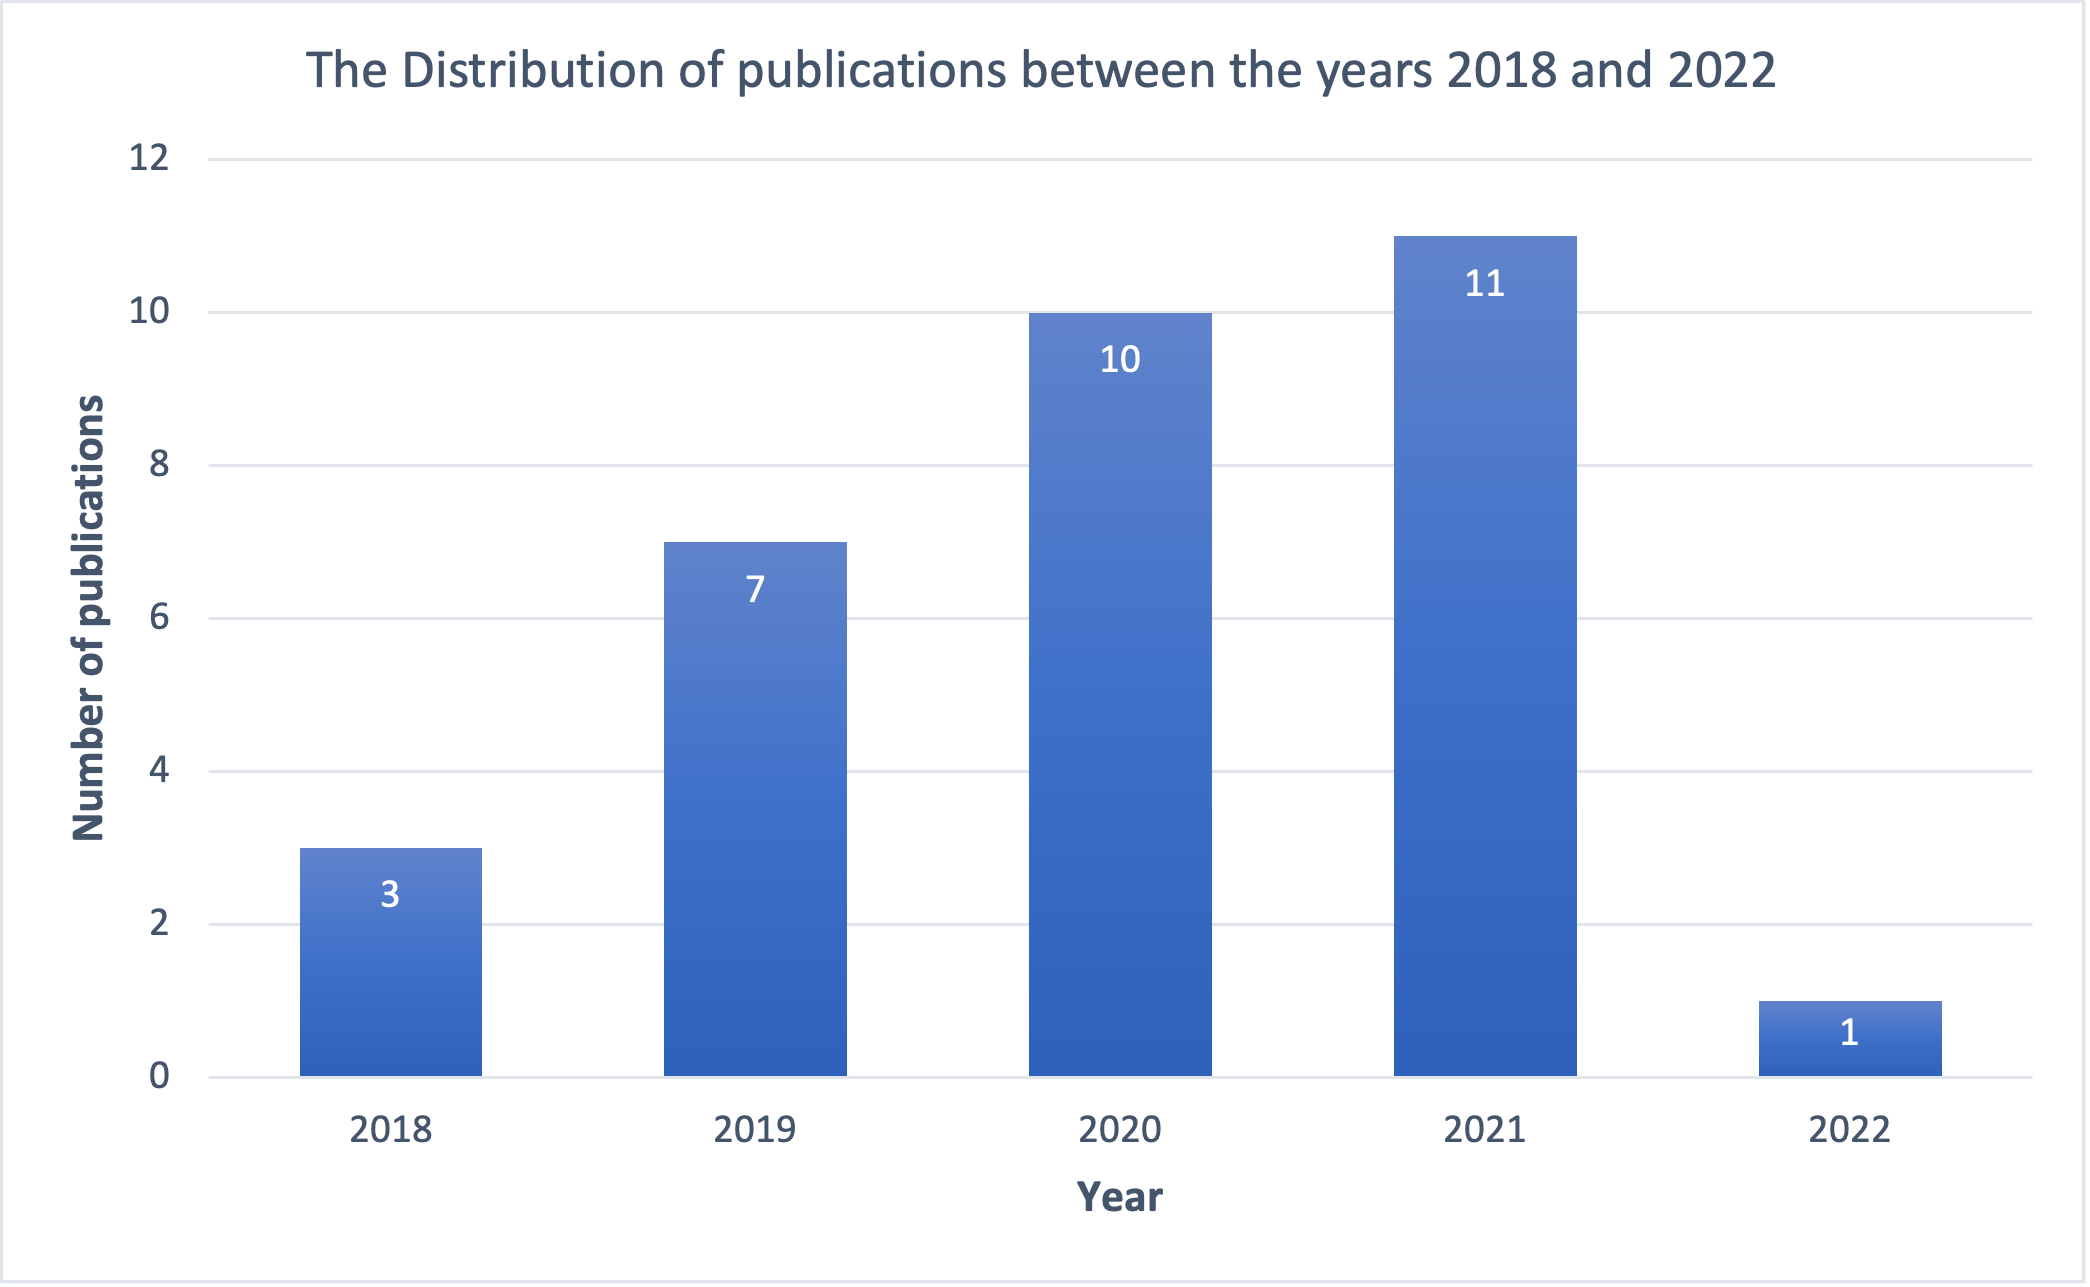
\includegraphics[scale=0.4]{Distribution_publications.png}
		\centering
		\caption{The Distribution of publications between the years 2018 and 2022}
		\end{figure}
		
		%Prediction level proportion
		To address \textbf{RQ2}, I need to look closely at the prediction level proposed in each paper. The work of \cite{original} categorized three prediction levels, i.e., Numeric Predictions,   Categorical Predictions, and Next Activities Predictions. Here I followed the same principle and categorized my final article. I calculated thae proportion of each prediction level and plotted the following graph.
		
		
		\begin{figure}
		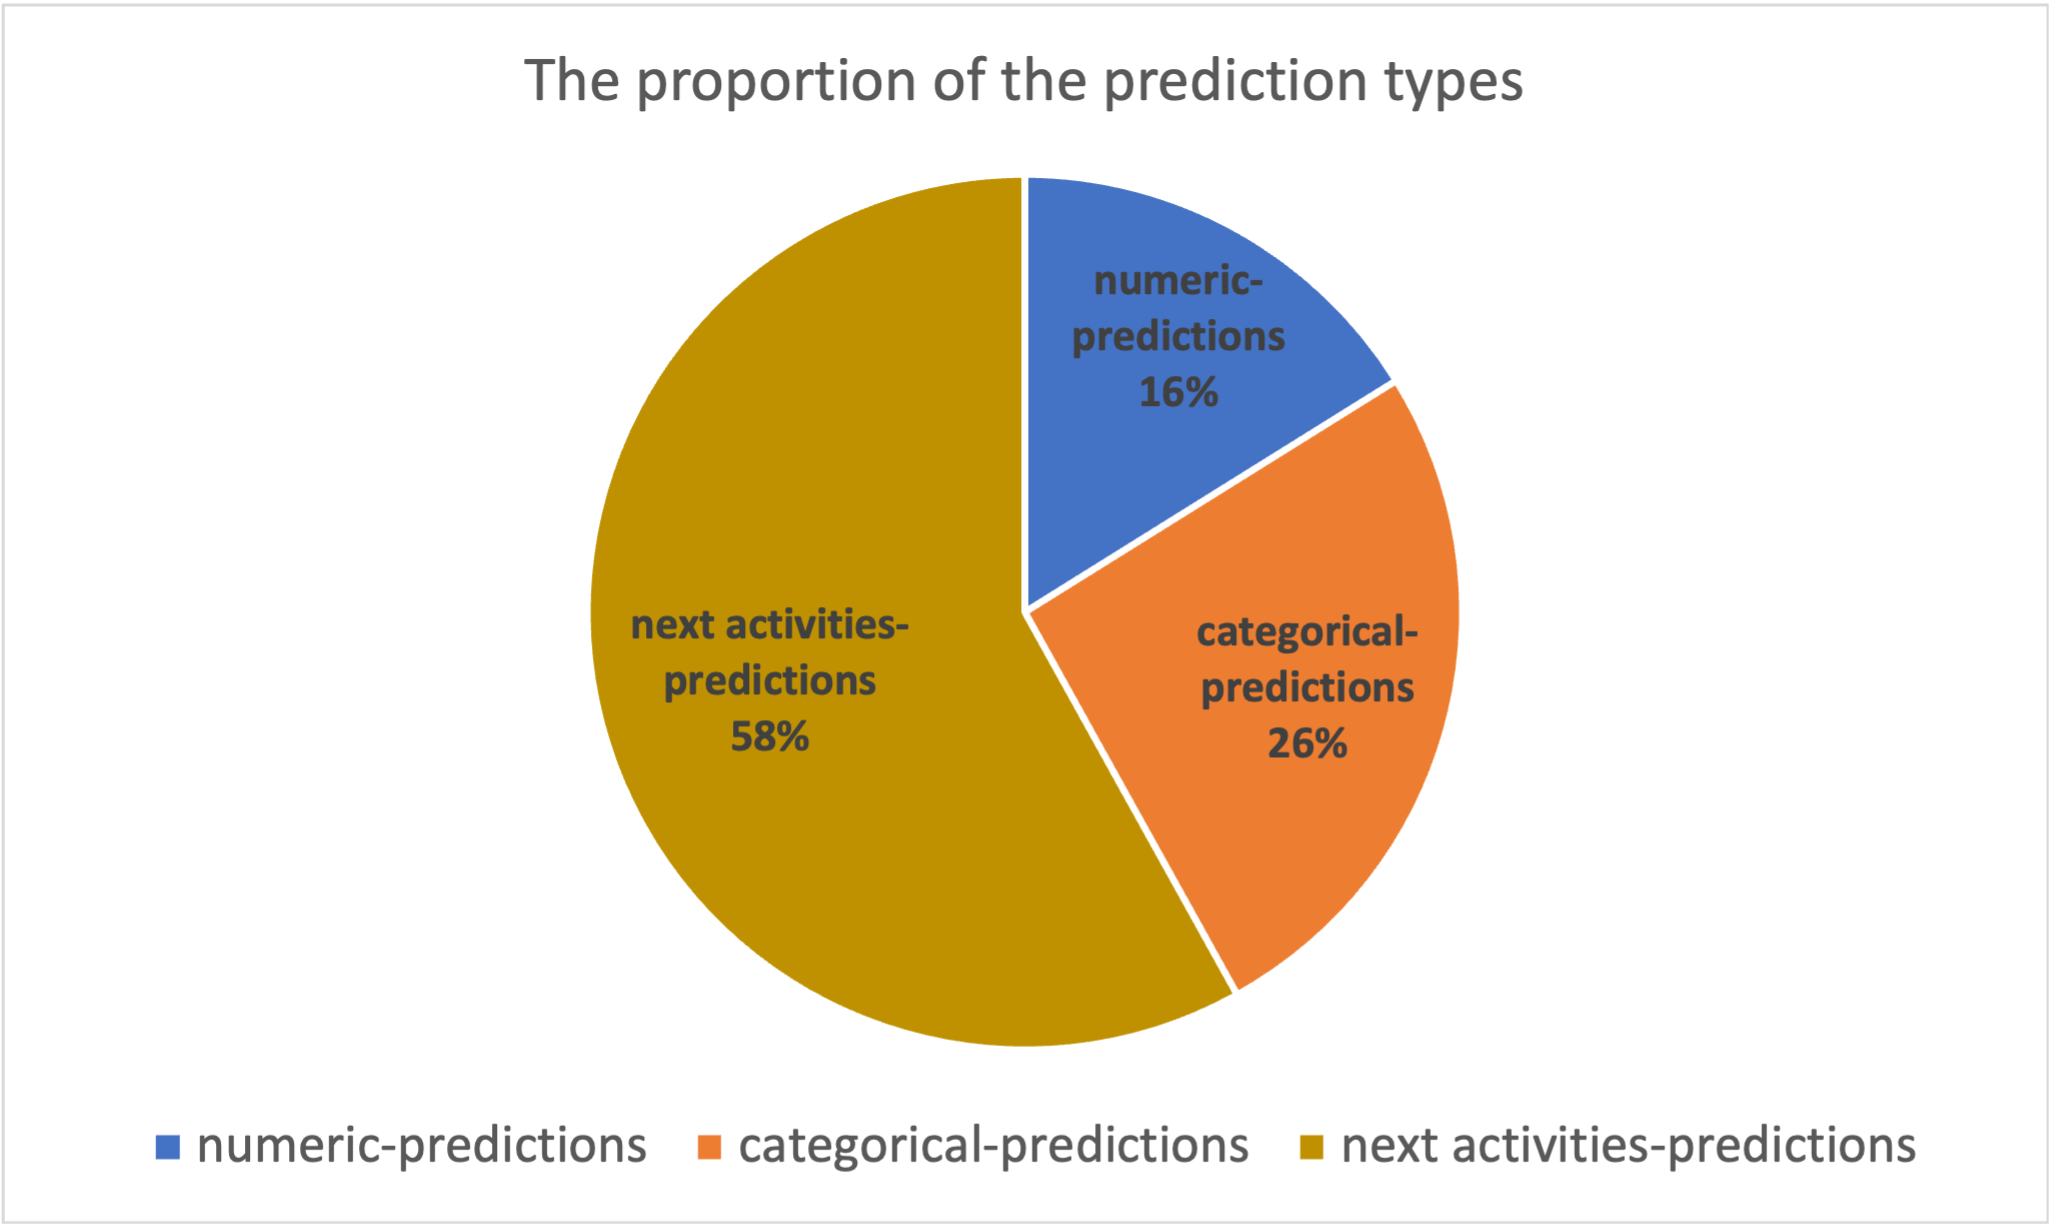
\includegraphics[scale=0.5]{proportion_prediction.png}
		\centering
		\caption{The proportion of the prediction types}
		\end{figure}
		
		People can observe that 55\% of techniques make a next-activity prediction. On the contrary, only 16\% of techniques make numeric predictions; I will look into this phenomenon in the following sub-sections. I will also summarize the benefits each prediction type brings to business logic as well as briefly talk about the algorithms and new trends that emerged in current studies.
		
		\subsection{Next Activities Predictions}
		
		\subsection{Categorical Predictions}
		
		\subsection{Numeric Predictions}
		%benefits os time prediction
		The work focuses on numeric predictions is another crucial area. However, the research papers published during the search period focus majorly on time prediction. Thus in this section, we will be concentrating only on the remaining time prediction. As demonstrated in \cite{art-13}, The prediction of the remaining time can be beneficial in areas where the scheduling and choice determination are involved. \cite{art-15} also addresses the significance of the remaining time prediction by mentioning its usage to avoid undesirable situations during the running business process. \cite{art-29} suggest that the remaining time should be communicated between business partners to provide the customer with better service. 
		
		The works in this area all rely on specific models. It is clear that different methods are used to make the prediction, but among them, neural networks are the most commonly used method. \cite{art-29} points out that the prediction of remaining execution time belongs to regression problems and \cite{art-17} illustrated that the Long Short-Term Memory networks (LSTMs) commonly perform better than other models. Due to these facts, it is not hard to imagine why neural networks are the most commonly used ones.
		
		%TODO:接下来分析不同文章中提到的方法以及有哪些创新
		
		
		
		
		
		
		%TODO: rewrite thentitle
		\section{Search on the algorithmical trend}
		
		To address \textbf{RQ3}, I have to take a deeper look into the algorithms used in each paper. 
		
		%首先介绍一下我们发现了哪些算法,哪些算法是主流,为什么;哪些算法不是主流,为什么。
		
		\begin{figure}
		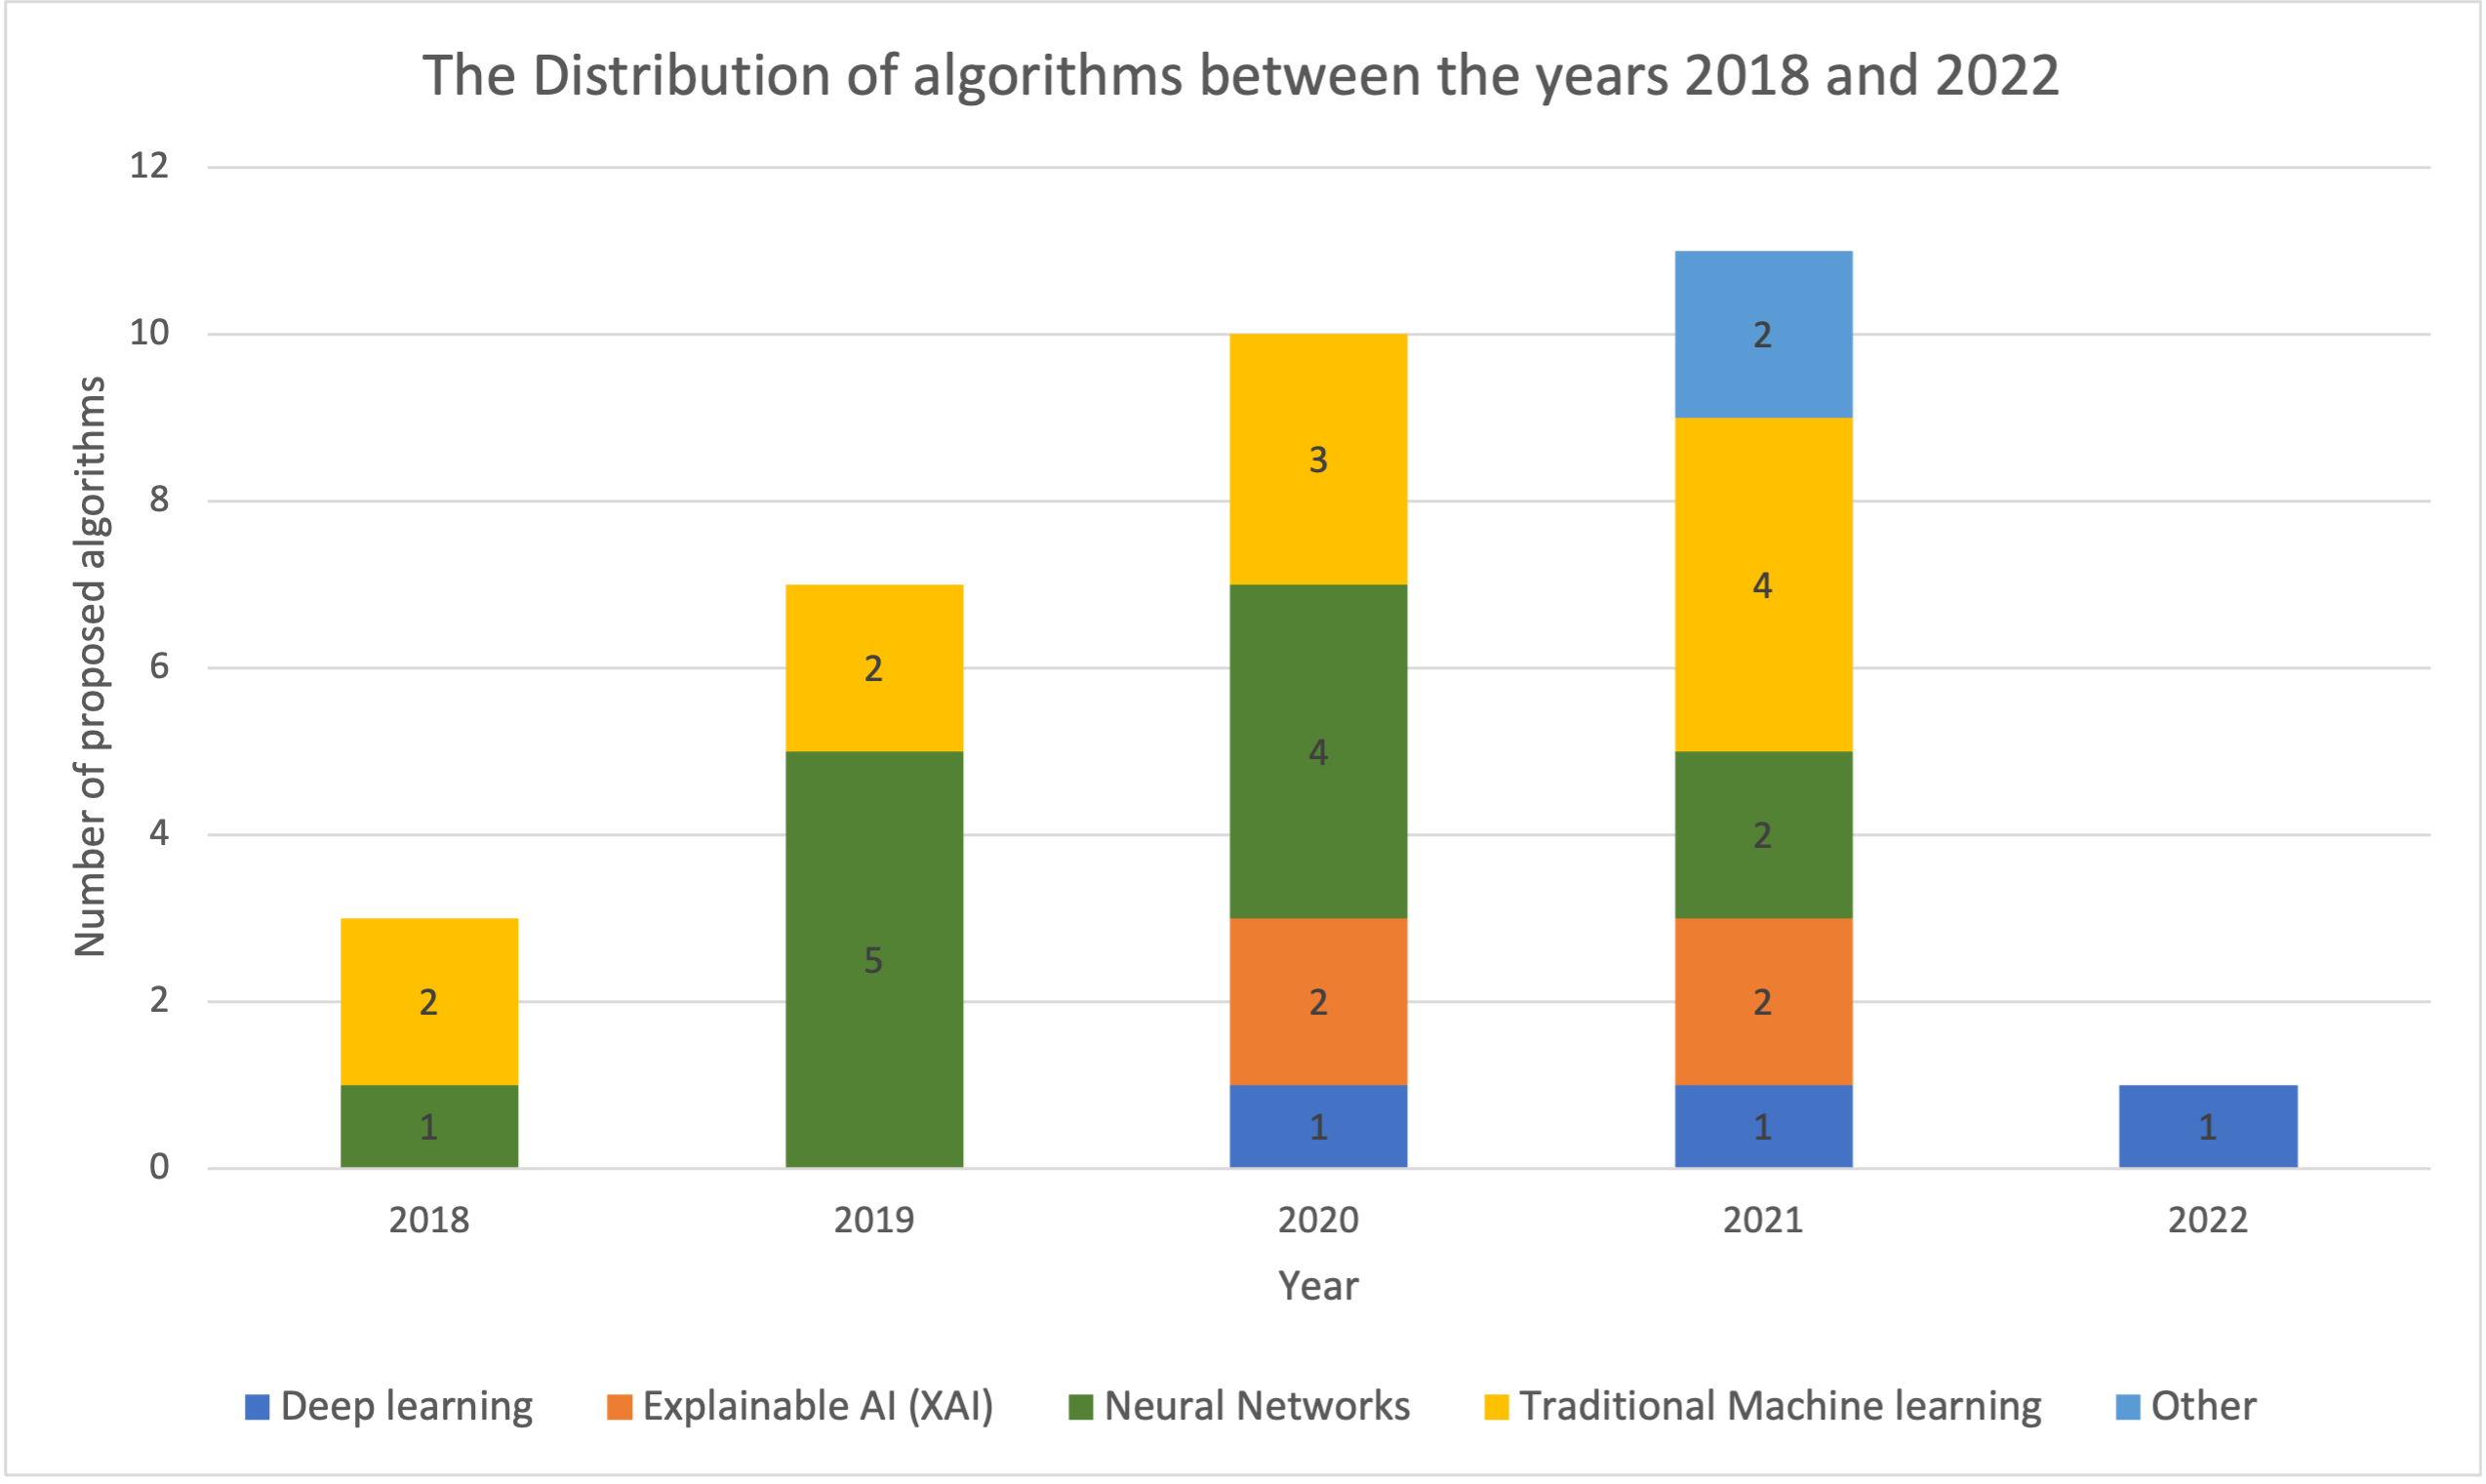
\includegraphics[scale=0.4]{Distribution_algorithms.png}
		\centering
		\caption{The Distribution of algorithms between the years 2018 and 2022}
		\end{figure}
		
		%算法的运用有什么新的趋势吗?XAI eg 为什么会有这种新的趋势
		%接下来研究一下为什么会有这种趋势,做一个新的图,研究可能的gap
		
		
		%可以介绍一下神经网络,解释一下什么是伸进网络,讲讲他的好处(精确),从他的不可解释性引申到XAI
		
		
		\section{Conclusion}




		
	\newpage
	\begin{thebibliography}{99}
	
	%TODO: 引用的格式???
	\bibitem{original}
	Di Francescomarino C, Ghidini C, Maggi F M, et al. Predictive process monitoring methods: Which one suits me best?[C]//International conference on business process management. Springer, Cham, 2018: 462-479.
	
	\bibitem{guidline}
	Kitchenham B. Procedures for performing systematic reviews[J]. Keele, UK, Keele University, 2004, 33(2004): 1-26.
	
	\bibitem{art-13}
	Ogunbiyi N, Basukoski A, Chaussalet T. Incorporating spatial context into remaining-time predictive process monitoring[C]//Proceedings of the 36th Annual ACM Symposium on Applied Computing. 2021: 535-542.
	
	\bibitem{art-15}
	Wahid N A, Adi T N, Bae H, et al. Predictive business process monitoring–remaining time prediction using deep neural network with entity embedding[J]. Procedia Computer Science, 2019, 161: 1080-1088.
	
	\bibitem{art-17}
	Galanti R, Coma-Puig B, de Leoni M, et al. Explainable predictive process monitoring[C]//2020 2nd International Conference on Process Mining (ICPM). IEEE, 2020: 1-8.
	
	\bibitem{art-29}
	Jian C, Xiaofu H, Qing Q. Selecting Publishing Points for the Optimal Sharing of Predictive Monitoring Information of a Service Process[C]//2019 IEEE International Conference on Web Services (ICWS). IEEE, 2019: 368-372.
		
	\end{thebibliography}

	
\end{document}
